%%%%%%%%%%%%%%%%%%%%%%%%%%%%%%%%%%
% Chapter 2 
%%%%%%%%%%%%%%%%%%%%%%%%%%%%%%%%%%
\chapter{Provenance Replay Software}
The Provenance Replay software, as implemented, attempts to meet the loose
requirements funded by the US National Cancer Institute’s Informatics Technology
for Cancer Research program (grant number 1U24CA248454-01). In addition, we
undertook an internal requirements engineering process, involving requirements
elicitation by focus group, and requirements validation using Technology
Acceptance Model (TAM) \parencite{davis_perceived_1989} and Net Promoter Score
\parencite{reichheld_one_2003} (NPS)-based survey instruments. These two
processes (initial development and requirements engineering research) will be
discussed in separate sections roughly corresponding to the chronological order
of the work, in which an Alpha release version of Provenance Replay was
developed first based on funding agency requirements and literature review, and
requirements engineering processes were used to refine software requirements and
validate the success of the initial implementation.

%%
%%
%%      1
%%
%%
\section{Overview}

As initially proposed, the aim of Provenance Replay is to “generate executable
code directly from a Result’s provenance” \parencite{caporaso_nci_2022}.
Framed as functional requirements:
\begin{itemize}
    \item Provenance Replay must ingest QIIME 2 Results, and from them produce command-line (BASH) and Python scripts
    \item These scripts must be usable with QIIME 2’s q2cli and Python 3 API interfaces
\end{itemize}

% EXAMPLE: don't indent "new paragraph" after itemize bullet list
\noindent Framed as a user story: \\
A QIIME 2 user, in a setting where new data must continuously be
merged with existing data, wants to parse a result from the previous iteration
of an analysis and use the resulting script to produce the same result after
incorporating the new data. 

I developed a Python package, \texttt{provenance\_lib}, to meet these basic
requirements.  The modular design targets two primary processes - the parsing of
provenance data from QIIME 2 Results, and “replay” tools which output executable
scripts, along with other reproducibility documentation designed to address the
challenges discussed above. These outputs are self-documenting, and leverage
UUIDs to make them identifiable as products of specific QIIME 2 Results. A third
module implements MD5 checksum-based validation of archive provenance, capable
of alerting a user to losses of integrity in their Results. 

This functionality was developed with human users as the primary constituency,
and implements both a Python 3 API and a command line interface. Reproducibility
scripts can be produced targeting the corresponding QIIME 2 Python 3 API and the
q2cli command line interface, allowing users to produce and consume Provenance
Replay outputs with their preferred interface. Though not the primary target,
design choices that support scaling and automation have been made where
possible, and replay commands offer many parameters to enable replay actions to
be faster and more resilient to compromises in data quality.

The following subsections explore the high-level architecture and select design
decisions made in the creation of this software.

%%
%%
%%      2
%%
%%
\section{Parsing provenance data from Archives}

The components of QIIME 2 Archives required for provenance parsing (e.g. the
VERSION files and the contents of the provenance directory) are consistently
formatted, with variations clearly defined and versioned in the QIIME 2 core
codebase. QIIME 2 guarantees that all Archives will contain a root directory
named with the archive UUID - this serves as the Archive’s identity, and I will
refer to it when needed as the “root UUID”. Within this root directory, all
archives contain a VERSION file, which holds the necessary information to
identify what version of the Archive Format specification this archive complies
with \parencite{qiime_2_development_team_anatomy_2018}. By determining which
archive version we are working with, it is possible to identify and parse all
files within the Archive which are relevant to Provenance Replay.

We will discuss the handling of various archive versions in greater detail
below. Here we will focus on the lower-level work of parsing the relevant data
from a version-5 Archive, the current and most complex Archive Format version.
(Figure \ref{fig:archive_structure})

\begin{figure}[htbp]
\centering
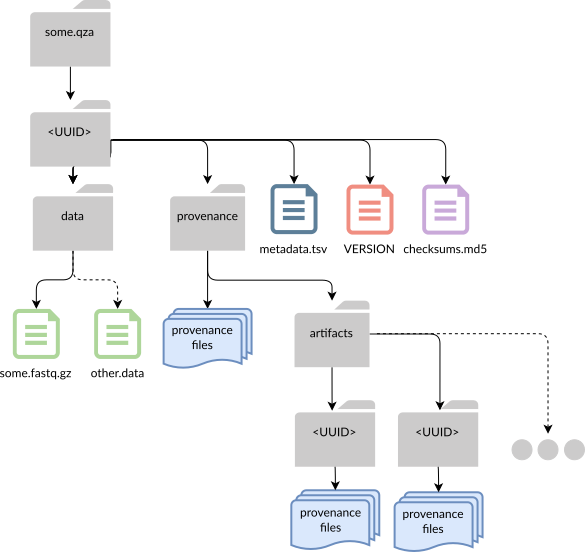
\includegraphics[width=\textwidth]{figures/archive_structure.png}
\caption[Diagram of the structure of a version-5 QIIME 2 Archive]%
{A graphical representation of the structure of a version 5 QIIME 2 Archive
stored as a Zip Archive. The directory structure is represented by gray
directory icons, with arrows indicating levels of nesting, wherein the parent
directory “points to” all of its contents. Single files are represented by the
“folded-corner” file icons, and a “file collection” icon in blue represents the
collection of files that contain provenance data. This is shown in an expanded
view in the following figure.}
\label{fig:archive_structure}
\end{figure}
A Result stored on disk as a zip file may have any filesystem-compliant
filename, and will be suffixed with .qza or .qzv by default. Internally, the
root directory is named with the UUID representing the Results stored within the
data directory. In a Version 5 Archive, the root directory contains an MD5sum
digest, a VERSION file detailing the Archive version and the version of the
QIIME 2 Framework that produced the Result, and a metadata.yaml file describing
primary characteristics of the Result itself. The data directory holds the
Result data, and the provenance directory contains captured provenance data.
Note that the artifacts directory may contain an arbitrary number of
provenance-files directories, and that these contain only provenance
information. By not capturing ancestral data in provenance, we reduce the risk
of unmanageably-sized Archives, at the “cost” of users needing multiple archives
to hold all of the data from a given analysis. Users generally manage this
complexity by organizing their Results in a file system, though more
sophisticated solutions are possible (e.g. a database mapping UUIDs to resource
IDs or locations on disk). (Figure \ref{fig:provenance_files})

\begin{figure}[htp]
\centering
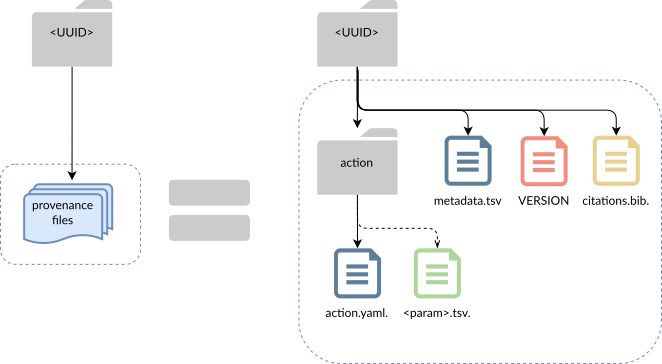
\includegraphics[width=\textwidth]{figures/prov_files.png}
\caption[Diagram of the provenance file directories in a QIIME 2 Archive]%
{An expanded graphical representation of the contents of a directory of
provenance files from a version 5 Archive. Each of these directories is uniquely
identified with the UUID of the ancestor result whose provenance is described
within. Information about the action that produced this Result is stored in an
action directory, including .tsv-formatted files representing any metadata used
in that action. Every provenance directory contains its own VERSION file,
metadata.yaml, and a bibtex-formatted list of relevant citations.}
\label{fig:provenance_files}
\end{figure}
VERSION files are specified in a simple, custom format. The root-level VERSION
file is checked for validity against a regular expression. If valid, the Archive
version is parsed using Python’s standard-library string manipulation methods,
and used to determine how to parse the rest of the archive. Bibtex files are
parsed with the bibtexparser library \parencite{boulogne_bibtexparser_nodate},
pandas (\cite{reback_pandas-devpandas_2020}; \cite{mckinney_data_2010}) is used to read the
metadata .tsv files, and pyyaml is used to handle the critical metadata.yaml and
action.yaml files.

A number of custom-defined constructors are required in order to parse these
YAML files, as pyyaml does not by default support serializing and deserializing
Python sets, or the QIIME 2-specific !cite, !color, !metadata, !no-provenance,
and !ref tags. The safe\_loader is used for all deserialization to reduce the
risk of malicious code injection.

Parsed provenance information for each Result is captured in a ProvNode object.
These serve as the data payloads in our provenance DAG. The ProvNode class is
implemented with a highly flexible initialization method, which initializes
component classes if the files they depend on are provided. ProvNode attributes
which depend on these component classes are frequently implemented using
Python’s @property decorator to allow for the possibility of absence, and the
ProvNode itself always has a property has\_provenance which downstream code can
use as a guard against nodes with no provenance data at all. In this way,
ProvNodes can be parsed from Results that have Archive Format versions with
varying levels of complexity. 

\begin{figure}[htp]
\centering
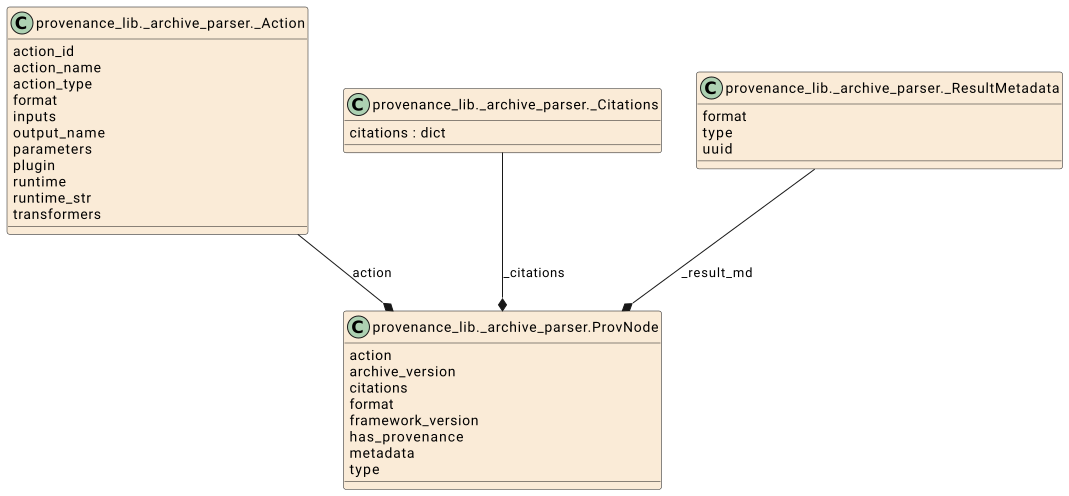
\includegraphics[width=\textwidth]{figures/ProvNode_UML.png}
\caption[UML Class diagram of the ProvNode class and its components]%
{A UML class diagram of the ProvNode class and its component classes, each of
which represents one of the key provenance files - action.yaml, citations.bib,
and metadata.yaml.}
\label{fig:ProvNode_UML}
\end{figure}

%%
%%
%%      3
%%
%%
\section{Cross-version analyses and handling no-provenance nodes}

The provenance parser attempts to represent provenance as completely as possible
given the available data. All known nodes are represented, regardless of whether
we have provenance data for them. Nodes without provenance data may exist, and
this impacts the construction of DAGs in some important ways.

If a V1+ archive was constructed to represent a Result R with at least one V0
Result (S) as an ancestor, then for some subgraph of the DAG representing R,
there is no provenance data to parse describing S. To be more specific, there
will be no provenance directory named with S’s UUID saved in R’s
provenance/artifacts directory. A record of S’s UUID will, however, be saved in
the action.yaml file of S’s immediate descendant.

DiGraph nodes are literally UUID strings. The minimal DiGraph node has the
following attributes:
\begin{itemize}
    \item has\_provenance - a flag indicating whether provenance data exists for this node
    \item node\_data - either a ProvNode payload, or None
\end{itemize}

The provenance parser, for completeness, must include a minimal node in the
DiGraph constructed to represent R during initial parsing. For safety in working
with these graphs, archive parsers first construct ProvNode payloads for nodes
which have provenance, add any no-provenance nodes to the graph, and then check
each node for the absence of a provenance payload, setting the required
attributes in cases where they are missing. Consumer functions may safely
(without KeyError) check whether a node has\_provenance, and access ProvNode
properties appropriately if provenance exists.

%%
%%
%%      4
%%
%%
\section{Provenance Parsers and Dispatch for provenance parsing}

Provenance Replay implements an extensible dispatch system for parsing
provenance. All parsing is done by implementations of an abstract base class
Parser, which defines the basic contract for any provenance parser. 
\begin{itemize}
    \item A Parser implements the classmethod get\_parse, which ingests arbitrary input data. It either returns a Parser that can parse that data, or it raises an Error.
    \item A Parser implements the method parse\_prov, which ingests an appropriate data payload, parses it, and returns a ParserResults object.
    \item A Parser has a string attribute accepted\_data\_types required for the production of error messages when the parser receives a type of data it cannot parse.
\end{itemize}

Parsers that meet this contract may be registered in parse.select\_parser.
Briefly, parsing proceeds as follows. A user calls the ProvDAG class, which is a
domain-specific wrapper around a networkx.DiGraph, with some input data.
ProvDAG.\_\_init\_\_ uses the parse\_provenance function, which calls
parse.select\_parser with the input data. This function iterates over the known
parsers, testing the data payload against their get\_parser methods and
aggregating the errors that result. 

If a Parser that can parse the payload is found, that parser will be returned
immediately, and aggregated errors will not be reported. The returned Parser
instance’s parse\_prov method parses the input data payload and returns a
ParserResults object. A ProvDAG is then initialized from the DiGraph and other
data contained in the ParserResult, exposing user-facing methods for accessing
and manipulating the aggregated provenance data.

ParserResults objects function as a common data interface between the Parsers
which create them, and the ProvDAG class. (Figure \ref{fig:ParserResultsUML})

\begin{figure}[htp]
\centering
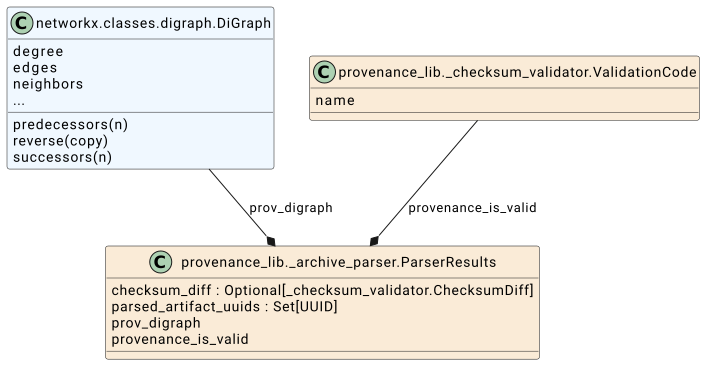
\includegraphics[width=\textwidth]{figures/ParserResultsUML.png}
\caption[UML Class diagram of the ParserResults class and its components]%
{A UML class diagram of the ParserResults object with associated properties.
Classes in beige are locally defined, while classes in blue are imported from
NetworkX.}
\label{fig:ParserResultsUML}
\end{figure}

If no adequate Parser is found, an UnparseableDataError is raised, and the user
receives a digest of error outputs which they can use to troubleshoot their
input data. Should external tools make use of provenance parsing, this custom
error type may simplify graceful error handling in cases where it is more
important to continue processing input data than to consider/correct failed
input data. 

Four “top-level” Parser implementations currently handle all parsing needs.
These are:
\begin{itemize}
    \item ProvDAGParser: parses a ProvDAG object, enabling the copying of ProvDAG objects
    \item EmptyParser: parses None enables the creation of empty ProvDAG objects
    \item ArchiveParser: parses a single QIIME 2 Archive
    \item DirectoryParser: parses a directory of QIIME2 Archives, returning a single ParserResults object which represents all parsed Archives in a single DiGraph
\end{itemize}

Parsers are responsible for deciding whether they can parse a data payload, and
are not required to return an instance of their own class. This flexibility
allows for the extension of individual Parsers to handle an arbitrary number of
related data types. For example, if ArchiveParser.get\_parse() receives any type
or version of QIIME 2 Archive, it will handle dispatch internally, returning an
instance of a child class of ArchiveParser designed to address the specific
needs of that type or version of Archive.

This architecture reduces coupling between the high-level parse\_provenance
function (and its callers), and the low-level parsing code, by replacing direct
dependencies with dependencies on a shared abstraction (Parser). Modifications
to existing Parsers are immaterial to the high-level code, and extending the
codebase with an additional “top-level” Parser requires only the implementation
and registration of the Parser. 

\begin{figure}[htp]
\centering
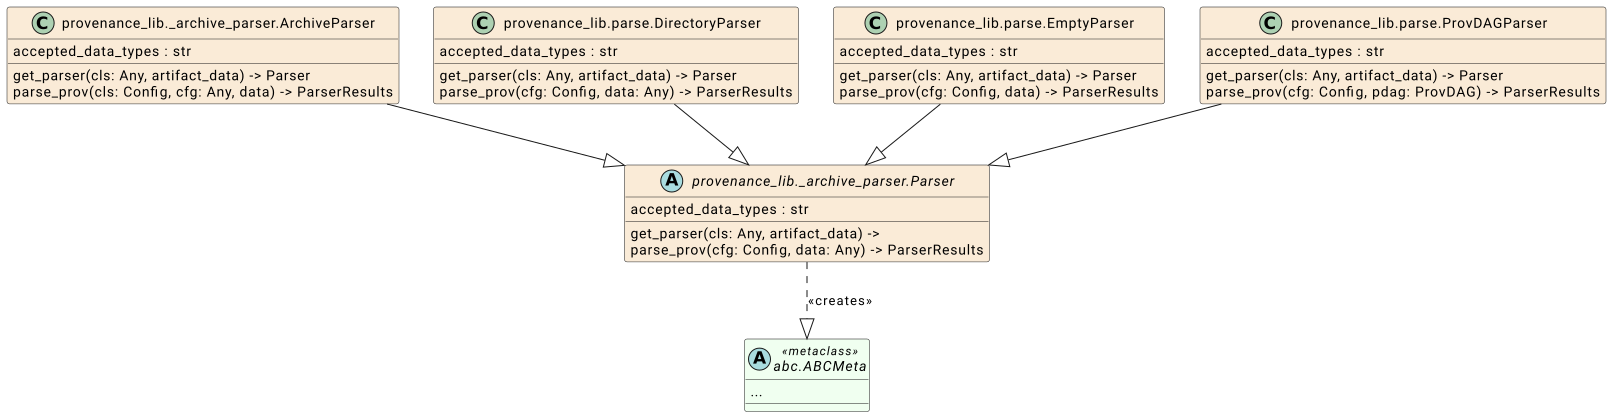
\includegraphics[width=\textwidth]{figures/allParsersUML.png}
\caption[UML Class diagram of the abstract Parser class and its implementations]%
{This UML class diagram describes the abstract Parser class and its top-level
implementations. The element notation “C” to the left of the class name
indicates a class, while “A” indicates an abstract class. Classes in beige are
locally defined, while classes in light green are imported from the standard
library. Note that many additional, specialized Parser implementations are
accessible through e.g. ArchiveParser.get\_parser.}
\label{fig:allParsersUML}
\end{figure}

%%
%%
%%      5
%%
%%
\section{Handling Changes in Archive structure over time}

The QIIME 2 Framework defines six Archive Format versions, numbered from 0 to 5,
which have increased in complexity as provenance capture has become more robust.
Results created in the earliest of these Archive Formats (v0) do not contain
provenance data at all. I have covered the details of these archive structure
changes at length in the developer documentation \parencite{qiime_2_development_team_archive_2018},
so will focus on the architectural decisions made to support this structure in
Provenance Replay.  Archive Formats are explicitly versioned, because change is
anticipated and must be supported, so extensibility is a key non-functional
requirement.

Archive parsing proceeds roughly as follows.
\begin{enumerate}
    \item The parser uses filename data stored in its class attributes to identify all file paths present that should be parsed. These are grouped by Result.
    \item If any expected files are missing, the parser responds appropriately (e.g. raise/warn).
    \item The parser instantiates a ProvNode object for each Result by calling ProvNode with a collection of Result-specific filepaths.
    \begin{enumerate}
        \item[3.1.]ProvNode.\_\_init\_\_ iterates over whatever filepaths it receives, dispatching the actual parsing to appropriate helper functions. 
    \end{enumerate}
    \item The parser builds a DiGraph representing the provenance history of the Archive
    \item The parser returns a ParserResults containing this DiGraph and other attributes
\end{enumerate}

This approach forefronts extensibility through flexibility and encapsulation.
The ProvNode initializer is a generalist with no knowledge of the requirements
of the Parsers. Its single responsibility is to instantiate ProvNodes from the
data it receives, and it doesn’t need to know anything about archive versions -
only where to dispatch different files for parsing. If it gets the file, it
parses it. Parsers, on the other hand, are format-specific, and are responsible
for checking the integrity of their input data against their understanding of
the Archive Format version they target, collecting files and sending them out
for parsing, and returning the resulting ParserResults object.

To date, changes to Archive formats have generally been additive, and have
accreted in relatively small increments, which as a general trend lends itself
well to inheritance. In order to support a new Archive Format (v6) that captured
a new type of provenance file with every Result, we might only need to:
\begin{itemize}
    \item Define a class or function capable of the low-level parsing (e.g. loading serialized data)
    \item Add a check for the new file to ProvNode.\_\_init\_\_(), calling this class/function
    \item Subclass Parserv5, adding the new filename to the expected\_files\_in\_all\_nodes class attribute
\end{itemize}

% EXAMPLE: Caption to the right side of Figure
\begin{figure}[htp]
    \begin{minipage}[c]{0.5\textwidth}
        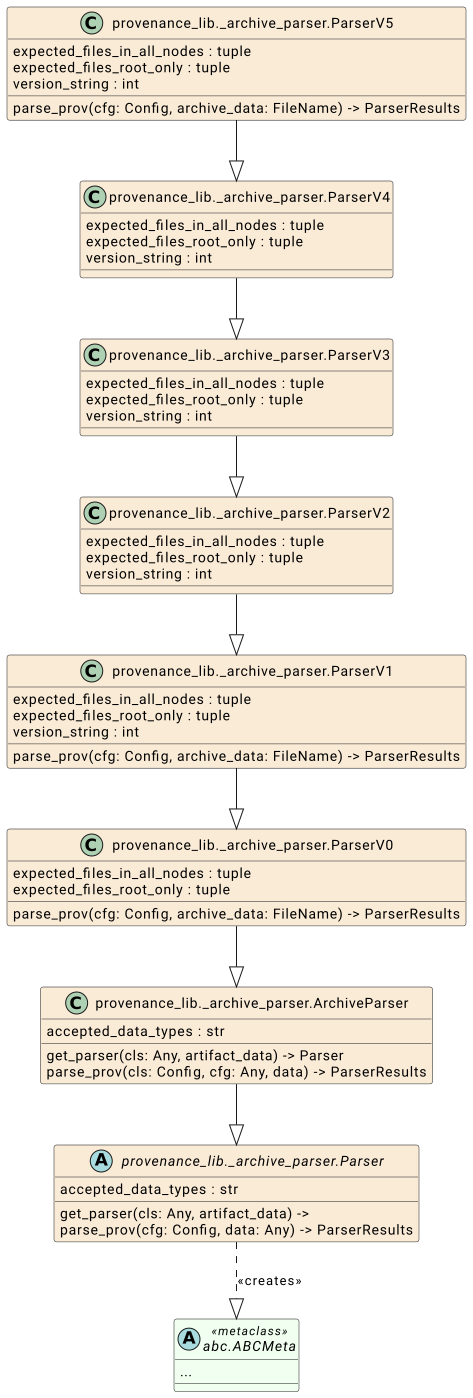
\includegraphics[width=\textwidth]{figures/archiveParserUML.png}
    \end{minipage}\hfill
    \begin{minipage}[c]{0.45\textwidth}
\caption[UML Class diagram of the Version-specific Archive Parsers]%
{This UML diagram depicts select features of the \_archive\_parser module. Classes
in beige are locally defined, while classes in light green are imported from the
standard library. The element notation “C” to the left of the class name
indicates a class, while “A” indicates an abstract class. The inheritance
structure used in the definition of version-specific archive parsers mirrors the
archive format definition itself in the QIIME 2 Framework, and dramatically
reduces the amount of redundant code, resulting in a smaller maintenance surface
area. Note that the get\_parser implementation in the ArchiveParser class can
return instances of any of the child parser implementations, and the parse\_prov
implementation in Parserv1 is used by all of the classes that depend on it.
Changes in parser behavior from V1-V5 are effected through simple changes in
class data, and ‘private’ helper methods like \_validate\_checksums}
    \end{minipage}
    % \label{fig:allParsersUML}
\end{figure}

Low-level parsing/loading work is handled by file-type-specific classes, which
load some type of data, and expose key values or behaviors as object properties
or methods. Strict validation of file contents is not performed (though it would
certainly be possible to do so). With the exception of a few key characteristics
(UUID, archive version number, etc.), the contents of these files are important
to the end user, but not to the Provenance Replay tool itself. By parsing and
providing all contents without, for example, schema validation, we can meet end
user needs with simpler and therefore more performant code.

This implementation allows some classes of extension to be made primarily by
manipulating class attributes, resulting in a minimal maintenance surface area.
Changes made to the structure of the action.yaml file in versions 2, 3 and 4
required no changes to the parser logic. The addition of a citations.bib file to
all Results in version 4 proceeded as described above. The addition of a
checksums.md5 file in the root directory for V5 required this process, plus the
re-implementation of a helper function, and a call to super().parse\_prov. The
code for all of these Parsers is minimal, as nearly all behavior is inherited. 
(Figure \ref{fig:parserCodeBlock})

% TODO: This ref ^ is borked, pointing to the prior figure

\begin{figure}[htp]
\centering
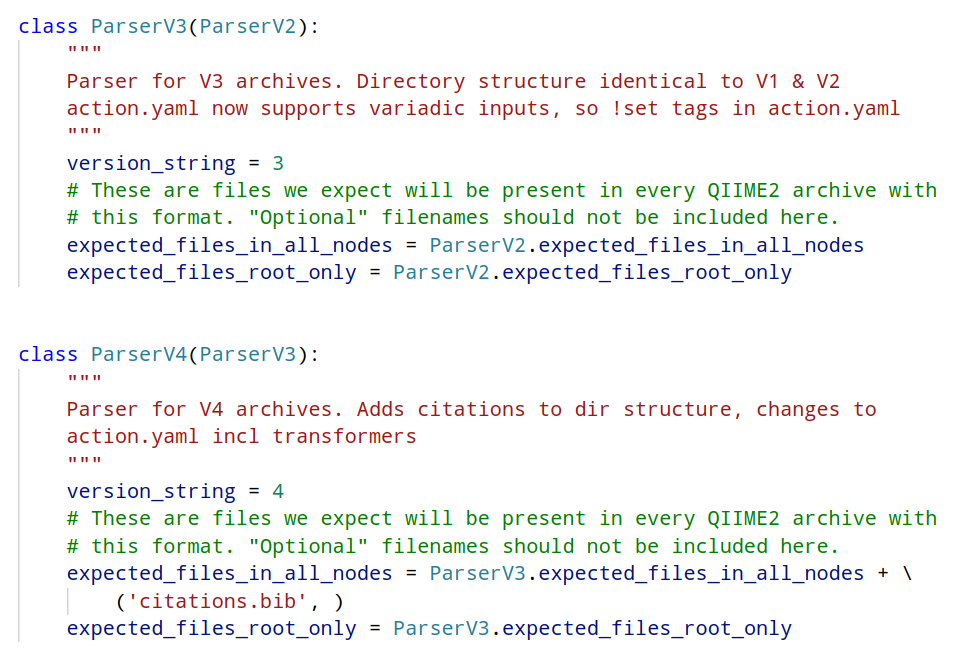
\includegraphics[width=\textwidth]{figures/parserCodeBlock.png}
\caption[Code snippet illustrating the value of inheritance to ArchiveParser Versions]%
{full code of the ParserV3 and ParserV4 classes, illustrating the value of
inheritance and low-level parser flexibility in reducing code surface area.}
\label{fig:parserCodeBlock}
\end{figure}

%%
%%
%%      6
%%
%%
\section{Representing single Results or full analyses with DiGraphs}

Many studies require information from more than one QIIME 2 Result in order to
adequately address their research questions. We must therefore support user
stories in which a user replays multiple Results into a single “analysis-level”
script. Failure to do so would result in users generating multiple replay
scripts with potentially high levels of duplication, and then manually or with
their own software tools, a) incurring unnecessary computing costs to generate
and then delete many duplicate Results, or b) incurring unnecessary researcher
or developer costs to merge these replay scripts for a single run without
duplicate Results. Either of these would likely be prone to user error. 

The provenance of a single QIIME 2 Result conforms to the properties of a
directed acyclic graph (DAG), with one or more “input” nodes and a single
terminal node representing the “root” node whose data is contained in the
Archive. Each node in the graph represents a Result, and each edge u → v
represents an action that took node u as an input and produced node v as an
output. A node can only be the product of one Action, so multiple in-edges to a
single node will always represent the same Action. We capture Action-specific
data in the graph nodes produced by that action, for loose parity with the
representation of that data in both the Archive structure and in the widely used
q2view provenance graph visualization. 

These DAGs are implemented as DiGraph objects, defined by the NetworkX library
for graph analysis. NetworkX was selected for many reasons. It is widely-used
and well-supported, offers most common graph operations built in, and supports
export to common graph visualization libraries (e.g. Cytoscape). There are a
number of significantly more performant graph libraries available for Python,
but as a pure Python library NetworkX presents a reduced risk of dependency
management challenges.

In our implementation, DiGraph nodes are literal UUID strings, with provenance
information stored as node attributes. NetworkX supports the creation of graphs
with user-defined hashable objects as nodes, but our approach results in a graph
in which common interactions with nodes (e.g. querying the graph, asserting
against node properties) are simpler and more intuitive.

QIIME 2 provenance data folders are archived in a non-hierarchical format for
reasons of simplicity and ease of access. Every parent Result’s provenance is
stored in its own UUID-named directory, and these are all placed into a single
parent directory. Creating a DiGraph, then, requires us to parse the provenance
data in each of these provenance directories, capturing ancestry information
about each node, and using it to define the edges that connect a node to its
input dependencies.

QIIME 2 Results are stored in independent Archives, and each archive contains
only the provenance data directly relevant to its own creation. It is common for
two Results from a single analysis to share many, or even all of their data
dependencies. DAGs with multiple terminal nodes are common, making the DAG a
natural fit for representing complete QIIME 2 analyses, with an arbitrary number
of import nodes, and an arbitrary number of terminal nodes. NetworkX DiGraphs
support arbitrary numbers of disconnected subgraph components, allowing the
DiGraph data structure to accommodate many different needs. 

Users may parse a single Result, many nested directories of Results from a
single analysis (i.e. which share a common history), and even multiple Results
from unrelated analyses (i.e. disconnected subgraphs with no common history).
This simplifies the handling of nodes from Archive Format versions that did not
support provenance capture, while providing users interested in graph topologies
with the ability to interrogate the structure of their parsed provenance DAGs.
It is, for example, trivial to determine whether a provenance DAG is composed of
one continuous, or many discontinuous subgraphs.

%%
%%
%%      7
%%
%%
\section{Graph Union}

Because provenance data is captured in a decentralized (per-Result) way, the
ability to union two DiGraphs is fundamental to our ability to efficiently
represent complete QIIME 2 analyses. By implementing a ProvDAG.union method,
individuals who need fine-grained control can manually assemble a DAG from
arbitrary Results. Union is also used internally in the DirectoryParser, which
traverses a (potentially nested) directory structure parsing individual Results
if they are not already represented in the DAG under construction, and unioning
them into a whole.

NetworkX implements a number of “union-like” operations on DiGraphs, and
DiGraph.union itself is not appropriate for our common use cases, because it
requires that the joined subgraphs be disjoint. ProvDAG.union wraps
DiGraph.compose\_all, which does not impose this requirement, and allows for the
joining of an arbitrary collection of DiGraphs.

ProvDAG objects capture significant data in addition to the DAG itself,
including the root UUIDs of all Results passed in for parsing, collections of
terminal UUIDs, and information about the validity of the DAG’s provenance. As a
result, some additional processing is required for safe graph union. Parsed
Result UUIDs and ChecksumDiff objects are aggregated, preserving the most
possible information. Status descriptions like the provenance ValidationCode are
handled by taking the minimum. A ProvDAGs validity level is represented as the
minimum of the validity level of all of its component Results.

%%
%%
%%      8
%%
%%
\section{Graph views for graph manipulation}

QIIME 2 implements three types of Action. One of these, the Pipeline, operates
by coordinating the execution of multiple other QIIME 2 Actions, and outputs the
Results produced by all of these “nested” Actions. Pipelines may be nested to an
arbitrary degree, making visual disentanglement of these nesting relationships
unwieldy.

To support completeness, QIIME 2 captures provenance information for all of
these Actions - the Pipeline itself, and the nested Actions it executes. As a
result, both user-passed and pipeline-passed parameter sets are captured in
separate UUID-named directories in provenance. When Pipelines are run, multiple
directories representing the same Result exist in provenance. Pipelines have an
alias-of field referencing the UUID of the nested Result within their
action.yaml file, allowing us to associate Pipeline Results with the provenance
of their internal Actions. 

Again for reasons of completeness, Provenance Replay’s Archive parsers include
all captured provenance data in the ParserResults objects they return. We can
call this the complete view of provenance. Many use cases require subgraphs,
which we implement with NetworkX GraphViews \parencite{hagberg_exploring_2008}.
These are lightweight read-only subgraphs generated from the complete DiGraph,
which allow us to exclude sets of unneeded nodes without actually removing them
from the original data structure.

Most users, for example, are concerned only with the Actions they actually ran,
or would need to run to reproduce some analysis. In other words, they care only
about the Pipeline, and not the nested Actions the pipeline executes on their
behalf. During parsing, we capture the root UUID of each Result a user specifies
for parsing. These are stored as a set in an attribute on the ProvDAG. By
traversing the complete graph backwards through all direct ancestor nodes,
beginning from each of these UUIDs, we can build a set of all “outer” Results
that disincludes the nested “inner” nodes created without direct user
participation. We call this the collapsed view of provenance, and it represents
the minimal set of QIIME 2 Actions a user might run to produce the parsed
Results.

A third, expanded view of QIIME 2 provenance excluding Pipelines and including
all inner Actions may be targeted for future development \parencite[Issue #74]{keefe_issues_2021}.
This view has potential utility as a tool for deeper inspection of analytical
workflows, allowing users to study, modify, and re-run all of the fundamental
Actions being run by Pipelines. 

The collapsed view will be familiar to users of q2view, in which it is used to
present analysis provenance with a minimum of visual clutter (see Fig 1).
Support for this fundamental idea that different users might require different
views of provenance is extended to the Replay component of the software, in
which replay scripts are assembled using an input DiGraph. Though replay of the
collapsed view is currently hardcoded, this approach will make replaying an
expanded view of provenance straightforward when and if that view is
implemented.

%%
%%
%%      9
%%
%%
\section{Checksum Validation}

The md5sum digest stored in the Archive’s root directory during provenance
capture lists the relative file paths of all Archive contents, paired with MD5
hashes of each file.  By re-hashing all of the files in the Archive, Provenance
Replay allows us to confirm whether files have been added, removed, or changed
in the Archive since it was originally created. 

Checksum Validation is not intended as a tool for diagnosing intentional
falsification of results. checksums.md5 is an unsecured plain text file, which a
modestly savvy user with the intention to falsify results could update with MD5
hashes that match the tampered archive contents. Even were this not the case,
MD5 hashes are not cryptographically secure, so a committed party would likely
be able to hack results. Though cryptographic security is nice in theory, it
comes with logistical and computational costs that render it not a goal we are
currently working to support in QIIME 2.

QIIME 2 Results are saved to disk as simple ZIP files, and some advanced users
regularly interact with their data or history by extracting files from or
navigating through them, creating opportunities for inadvertent modification or
corruption. The primary utility of checksum-based archive validation is
two-fold. First, it allows us to identify archives that have been corrupted
unintentionally. Second, it supports basic troubleshooting of these archives, by
identifying which files have been added, removed, or modified. 

Checksum validation proceeds simply - all non-checksum-digest files in the
archive are hashed using hashlib.md5. The checksums.md5 file is parsed and a
diff is created, reporting which files were added, removed, and modified. This
re-hashing process could be time-consuming at large scale, so is optional. For
users who are interested in the validity of the Archives they work with, an
ordered scale of ValidationCodes has been established as an IntEnum. (Table \ref{tab:validationCodes})

\begin{table}[htp]
    \centering
    \begin{tabular}{|p{0.28\textwidth}|p{0.06\textwidth}|p{0.55\textwidth}|}
    \hline
    ValidationCode      & Enum value & Description                                          \\ \hline
    INVALID             & 0          & the Archive is known to be invalid                   \\
    VALIDATION\_OPTOUT  & 1          & the user opted out of checksum validation            \\
    PREDATES\_CHECKSUMS & 2          & V0-V4 Archives cannot be validated: assume validity  \\
    VALID               & 3          & the archive is known to be invalid                   \\ \hline
    \end{tabular}
    \caption[Defined ValidationCodes, ordered from least to most valid, with their descriptions]%
    {Defined ValidationCodes, ordered from least to most valid, with their descriptions}
    \label{tab:validationCodes}
\end{table}

\noindent In cases where Results must be compared, (e.g. graph union) the IntEnum
representation of these ValidationCodes allows us to use builtins like min() to
determine and capture the preferred level of validity.

%%
%%
%%      9
%%
%%
\section{Generating Executable Scripts with Provenance Replay}

Once provenance data has been parsed into a DiGraph (stored in a ProvDAG
object), we are able to “replay” that representation of analysis history into an
executable script. DAGs can, by definition, be topologically ordered, allowing
us to guarantee execution-order dependencies will always be satisfied. By
iterating over any topologically sorted provenance DAG, we can generate a script
that safely traverses from the initial import of data into QIIME 2 through to
the terminal Results.

Provenance replay relies heavily on the QIIME 2 Usage API, which offers a set of
tools for producing interface-specific examples of how Actions might be used
from interface-agnostic abstractions \parencite{qiime_2_development_team_usage_2018}.
The Usage API supports the generation of documentation, and also the execution
of Usage examples through a Usage class, which can be subclassed to support
specific interfaces and behaviors. In addition, the API defines a set of methods
which example authors can use to define examples.

In standard use, an author defines some data, and writes one or more usage
examples using these methods. Each component method of an example takes some
Usage instance (a “usage driver”) as its first input. Each usage driver defines
its own behavior, allowing the author to write a single example, which produces
varied results depending on which dependency is injected. These tools provide
the foundation for Replay behavior, which makes use of both “sides” of the API. 

The replay module provides user-facing actions for documenting parsed provenance
data, some of which programmatically define minimal usage examples. Users may
select from a hardcoded registry of supported usage drivers, which are injected
into the generated examples. Specifically, the injected usage driver, once
instantiated, is fed an ordered “chain” of calls to its initializer, import,
metadata, action, and comment methods, representing the topologically sorted
QIIME 2 Actions captured in a ProvDAG. The use.render method renders a script
output in memory, which is then written to the user-passed location on disk.

This module’s core functionality is exposed at the package level, and supports
the handling of both ProvDAG objects in-memory and one-shot parse-and-replay
operations through the Python interpreter. A command-line interface written with
Click \parencite{pallets_click_2014} in the click\_commands module exposes the
one-shot methods for use from the command line, and provides documentation and
tab-completion functionality.

%%
%%
%%      11
%%
%%
\section{Provenance Replay Usage Drivers}

Provenance replay relies on locally-defined usage drivers, implemented in
\_usage\_drivers, to support the production of QIIME 2 scripts. ReplayCLIUsage
targets the generation of q2cli scripts, and ReplayPythonUsage targets the
generation of Python 3 API scripts. Both drivers target script rendering. Though
example execution should work in theory, the examples generated by replay do not
support this behavior, as will be discussed later.

Both drivers subclass existing usage drivers imported from the Framework, but
deviate from them significantly in both requirements and behavior. The key
distinction results from differing assumptions about how examples are used, and
what data is available. The parent classes primarily support human users in
off-line contexts where fast failure is a positive outcome. The
locally-implemented drivers primarily support machine users, can trust that
examples produced from machine-generated data are syntactically correct, and
support successful execution even in contexts where the machine-generated data
don’t align perfectly with the user’s current computing environment. 

Provenance replay cannot, and should not have to, guarantee the availability of
the original raw data. Users may replay a script for many reasons - study,
extension to new data, extension to new applications, etc - and may not have
access (or need access) to the original data inputs. Support for “touchless”
corroboration of results with input data available is a useful future target,
but presents additional, external challenges which will be addressed below. As a
result, replay scripts are by default slightly incomplete, providing annotated
input sections where users are directed to provide paths to raw data inputs.
Future tooling that incorporates data management into the QIIME 2 platform will
allow for the full automation of replay workflows in the future (see Section
5.5.1). For users that indicate they are working with new sample metadata,
sample metadata inputs are similarly annotated for easy search. In Python
scripts, these annotations intentionally produce syntax errors, as these cause
failure before any actions are run, reducing aggravation for users who might
otherwise attempt to run an incomplete analysis. An intended side benefit of
this is that failures to provide required data are much easier to locate in text
editors with syntax highlighting support, because language servers often make
syntax errors highly visible.

QIIME 2 and its plugins change over time, and captured provenance from a single
Result may represent an arbitrary number of software versions. In addition,
plugins may be added to or removed from a deployment at will. As a result, it is
impossible to guarantee that users of provenance replay will be working in a
QIIME 2 deployment that offers the same functionality as that used when
conducting the initial analysis. Dedicated tooling for environment management is
planned for future work (see Section 5.2). In the meantime, provenance replay
proactively checks for concordance between action/parameter names captured in
provenance, and those available in the current QIIME 2 deployment. In cases of
critical failure where replay is impossible, error messages are raised directing
the user to approaches for solving the problem. In non-critical cases, where
replay is possible but may result in a script that will not run in the local
environment, the script is annotated with a “TODO” comment at the affected line,
describing the issue and steps that should be taken to remedy it.

In order to support users in navigating these manual data inputs/modifications,
all provenance replay scripts begin with a header block containing instructions
for use. Proceeding through these in a stepwise manner, the script user will be
directed to all necessary changes. In addition, the header block reports the
date/time of replay, the version of provenance replay used, and a note that the
script is machine-generated. To support the identification of the artifacts used
to generate a given replay script, all parsed UUIDs are output in a footer block
appended below the script itself. Both header and footer production are active
by default, but may be disabled according to user preference.


%%
%%
%%      12
%%
%%

\section{Naming Results, and managing uniqueness within namespaces}

In order to generate multi-step executables, our generated scripts must pass the
outputs of prior actions into the inputs of later actions. At the Action level
within the ProvDAG, we know the UUID of the input data, but not the output name
generated by replay. By using a {UUID: output} mapping in which captured or
programmatically-generated output names are stored during each replay step, we
provide subsequent steps with access to output names by UUID.

Complicating this slightly, these output names must be unique. Failure to
guarantee uniqueness could result in variables or file names being overwritten,
causing data loss and script failure, or worse, the false appearance of script
success despite a failure of data integrity. I handle this with UsageVarsDict, a
modified UserDict in which keys are unique by virtue of being UUIDs, and values
are also unique, providing a one-to-one mapping of UUID to value.
UsageVarsDict.\_\_setitem\_\_ suffixes these values with \_n (where n is some
integer) whenever values are added. When potentially-colliding values are added,
n is incremented as needed until the collision is avoided. 

This serves as a UUID-queryable "namespace" of strings that can be passed to the
usage API to serve as unique variable names. In practice, potential {UUID: name}
pairs are added to the collection, during which process name is mutated for
uniqueness. The unique name is then retrieved by UUID, and passed to the usage
driver for use.

Action output-names were not captured in provenance prior to Archive Format
Version 2. When available, we capture the output-name from provenance. Absent
that, we fall back on the output’s registered semantic type.


%%
%%
%%      13
%%
%%

\section{Supporting Attribution with Citation Replay}

As with the production of reproducibility documentation, making scholarly
attribution “too easy not to do” provides both short and long-term benefits to
the state of science. By reducing the time cost of attribution to researchers,
we allow them to focus their efforts on the creative and inferential work they
are uniquely good at. By improving rates of attribution, we provide incentives
for the development of new, high-quality analytical software. 

The QIIME 2 Framework’s registration API allows plugins to register
bibtex-formatted citations to computational methods, and use of this feature is
widespread. As a result, the provenance DAG structure gives us the ability to
aggregate the citations from any arbitrary collection of QIIME 2 Artifacts.
Reporting all registered citations from an analysis is straightforward for the
computer.

The utility of this information is reduced by a high level of duplication. The
same citation will have a different unique key in different plugin versions,
resulting in tenfold duplication in some analyses. By default, I apply the
following heuristic approaches to deduplicate citations, resulting in a very low
level of duplication in practice:

\begin{itemize}
\item Capture each unique key no more than once
\item Capture each DOI no more than once
\item Remove records with exact duplication in all of the following content fields:
    \begin{itemize}
    \item Title
    \item Author
    \item Journal/Booktitle
    \item Year
    \item Pages
    \end{itemize}
\item All citations for the QIIME 2 Framework are ignored (for efficiency) and replaced by a single hard-coded citation.
\end{itemize}

The first two approaches are straightforward deduplication based on unique keys.
Content-based deduplication is handled through the creation of hashable
BibContent objects, with a hash representing all of the above fields, which are
stored and looked up in a set. Many fields are used, because false negatives
(i.e. self ≠ other) are preferable to false positives, which would result in
the inappropriate removal of non-duplicate citations.  QIIME 2 Framework
citations are often highly duplicated, and provenance captured from older
QIIME 2 versions cites the preprint rather than the final, peer-reviewed
publication. Using a hard-coded citation ensures that users don’t double-cite
the Framework, and properly cite the peer-reviewed article.

Citation replay tools for the Python API allow users to generate citations from
a ProvDAG in memory, or from a directory structure of files on disk. The replay
citations CLI command supports citation reporting from files on disk.

%%
%%
%%      14
%%
%%
\section{Metadata capture and reporting}

The Framework captures all sample metadata passed to an Action in that Action’s
provenance, in .tsv format. These metadata files may be useful investigative
tools for provenance replay users attempting to reproduce an unfamiliar analysis
with new data, as they can provide context about what types of metadata were
used in a given analytical process.

Provenance replay by default writes this captured sample metadata to disk so
that it is available for review or reuse. To support association between
metadata and the action in which it was used, all .tsv files are written in an
action-specific directory, named according to the scheme
plugin\_name\_action\_name\_n. Here, n (such that n ≥ 0) is an integer used to
disambiguate between identical commands by order. If q2-demux’s emp-single
command is used six times in an analysis, the metadata captured from the zeroth
run will be captured in the folder where n=0, and so forth.

%%
%%
%%      15
%%
%%
\section{Communicating user preferences internally with Config and ReplayConfig objects}

With a variety of potential users and use cases, these provenance parsing and
replay tools accept many parameters. These are required at all depths of the
call stack. The Config and ReplayConfig objects centralize all of these
user-passed parameters, providing developers with a useful organizational
abstraction, and reducing clutter in function signatures by replacing many flags
with a single Python object. 

%%
%%
%%      16
%%
%%
\section{Supporting publication with a reproducibility supplement}

In order to make the process of reproducibility documentation fast and easy for
users, I have implemented a wrapper function that parses provenance from one or
more QIIME 2 Results into a ProvDAG (if that provenance is not already a
ProvDAG), and then generates a zip archive package of key reproducibility
documents. At this time, this “reproducibility supplement” contains replay
scripts for all supported interfaces and a bibtex-formatted citation file. The
function can easily be extended to include parsed Result archives and study
metadata, and will in future include a “methods manifest”, as described in
Section 5.1.1. This implementation is both computationally more efficient
(requiring a single parsing step to produce all outputs), and provides a
streamlined way for users to package common supplemental materials for sharing
or publication.
